\chapter{Proposed Techniques}

\section{Combining RRT and EP/N}
\label{sec:RRT-EP/N}
As mentioned in section~\ref{sec:stateoftheart}, RRT variants produce
suboptimal solutions, which must later be post-processed for shortening,
smoothing or other desired characteristics. On the other hand, EP/N, 
presented in section~\ref{sec:EP/N}, can optimize a solution according to any
given fitness function. However, this algorithm is slower at finding a first 
feasible solution. In this section we propose a combined approach, that uses
RRT to find an initial solution to be used as starting point for EP/N,
taking advantage of the strong points of both algorithms.

\subsection{The Combined Strategy}

\subsubsection{Initial Solution}
EP/N as presented in section~\ref{sec:EP/N} can not find feasible paths in a
reasonable amount of time in any but very sparse maps. For this reason, RRT
will be used to generate a first initial solution, ignoring the effects produced
by dynamic objects. This solution will be in the initial population of the
evolutionary algorithm, along with random solutions.

\subsubsection{Feasibility and Optimization}
EP/N is the responsible of regaining feasibility when it is lost due to a
moving obstacle or a new obstacle found in a partially known or totally unknown
environment. If a feasible solution can not be found in a given amount of time,
the algorithm is restarted, keeping its old population, but adding a new
individual
generated by RRT.

\subsection{Algorithm Implementation}
\begin{algorithm}[ht]
    \caption{$\operatorname{Main}()$}
    \label{alg:rrtepn}
    \begin{algorithmic}[1]
        \STATE \(q_{\text{robot}} \leftarrow \text{is the current robot position}\)
        \STATE \(q_{\text{goal}} \leftarrow \text{is the goal position}\)
        \WHILE{\(q_{\text{robot}} \neq q_{\text{goal}}\)}
             \STATE \(\operatorname{updateWorld}(\text{time})\)
             \STATE \(\operatorname{processRRTEPN}(\text{time})\)
        \ENDWHILE
    \end{algorithmic}
\end{algorithm}

The combined RRT-EP/N algorithm proposed here works by alternating environment
updates and path planning, as can be seen in
algorithm~\ref{alg:rrtepn}. The first stage of the path planning (see algorithm~%
\ref{alg:processrrtepn})
is to find an initial path using a RRT technique, ignoring any cuts that might happen during
environment updates. Thus, the RRT ensures that the path found
does not collide with static obstacles, but might collide with dynamic obstacles in the future.
When a first path is found,
the navigation is done by using the standard EP/N as shown in algorithm~%
\ref{alg:epn}.

\begin{algorithm}[ht]
    \caption{$\operatorname{processRRTEPN}(time)$}
    \label{alg:processrrtepn}
    \begin{algorithmic}[1]
        \STATE \(q_{\text{robot}} \leftarrow \text{the current robot position}\)
        \STATE \(q_{\text{start}} \leftarrow \text{the starting position}\)
        \STATE \(q_{\text{goal}} \leftarrow \text{the goal position}\)
        \STATE \(T_{\text{init}} \leftarrow \text{the tree rooted at the robot position}\)
        \STATE \(T_{\text{goal}} \leftarrow \text{the tree rooted at the goal position}\)
        \STATE \(\text{path} \leftarrow \text{the path extracted from the merged RRTs}\)
        \STATE \(q_{\text{robot}} \leftarrow q_{\text{start}}\)
        \STATE \(T_{\text{init}}.\operatorname{init}(q_{\text{robot}})\)
        \STATE \(T_{\text{goal}}.\operatorname{init}(q_{\text{goal}})\)
        \WHILE{time elapsed \(<\) time}
            \IF{First path not found}
                \STATE \(\operatorname{RRT}(T_{\text{init}},T_{\text{goal}})\)
            \ELSE
                \STATE \(\operatorname{EP/N}()\)
            \ENDIF
        \ENDWHILE
    \end{algorithmic}
\end{algorithm}

\section{A Simple Multi-stage Probabilistic Algorithm}
\label{sec:RRT-LP}

In highly dynamic environments, with many (or a few but fast) relatively small
moving obstacles, regrowing trees are pruned too fast, cutting away important
parts of the trees before they can be replaced. This dramatically reduces
the performance of the algorithms, making them unsuitable for these classes
of problems.
We believe that better performance could be obtained
by slightly modifying a RRT solution using simple obstacle-avoidance
operations on the new colliding points of the path by informed local search.
The path could be greedily optimized if the path has reached the feasibility
condition.

\subsection{A Multi-stage Probabilistic Strategy}

If solving equation~\ref{eq:problem} is not a simple task in static environments,
solving dynamic versions turns out to be even more difficult. In dynamic path planning
we cannot wait until reaching the optimal solution because we must deliver
a ``good enough'' plan within some time restriction. Thus, a heuristic approach
must be developed to tackle the on-line nature of the problem. The heuristic
algorithms presented in sections~\ref{sec:ERRT}, \ref{sec:DRRT} and~\ref{sec:MPRRT}
extend a method developed for static environments, which produces poor response
to highly dynamic environments and unwanted complexity of the algorithms.

We propose a multi-stage combination of simple heuristic and probabilistic techniques
to solve each part of the problem: Feasibility, initial solution and optimization.

\begin{figure}[ht]
\begin{center}
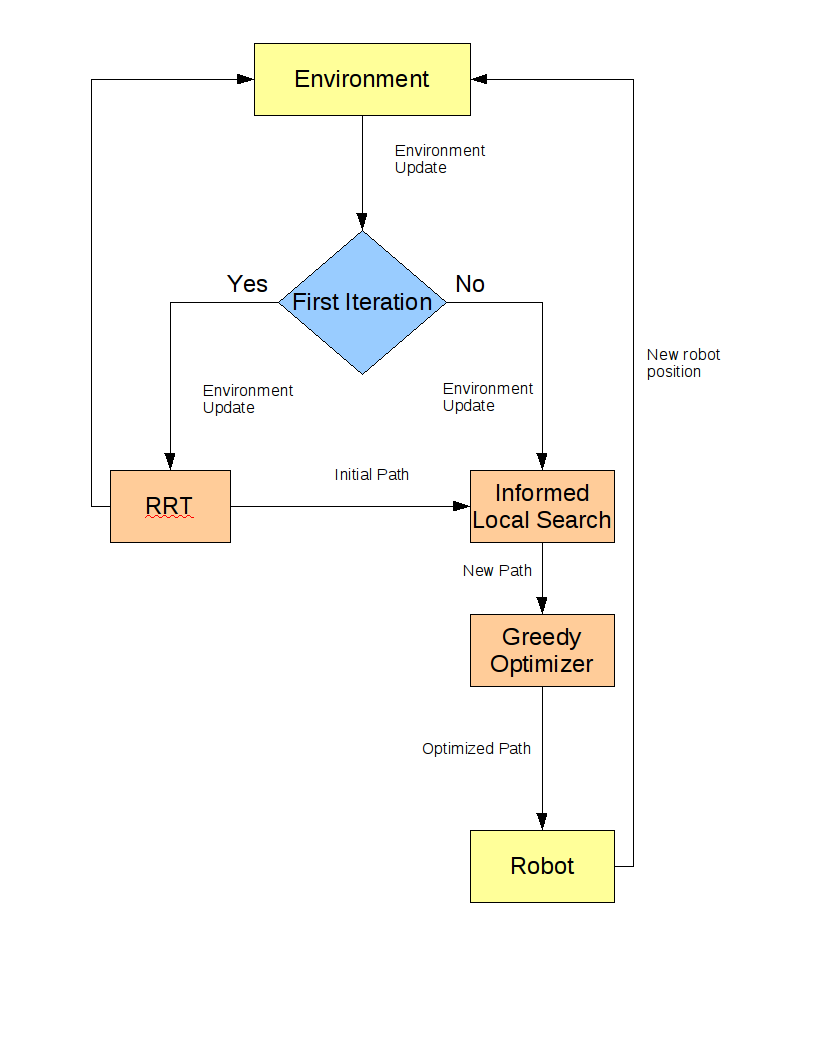
\includegraphics[width=0.6\textwidth]{images/diag}
\caption[A Multi-stage Strategy for Dynamic Path Planning]{\textbf{A Multi-stage Strategy for Dynamic Path Planning}. This figure describes
the life-cycle of the multi-stage algorithm presented here. The RRT, informed local search, and greedy heuristic are combined
to produce a cheap solution to the dynamic path planning problem.}
\label{fig:diag}
\end{center}
\end{figure}


\subsubsection{Feasibility}
The key point in this problem is the hard constraint in equation~\ref{eq:problem}
which must be met before even thinking about optimizing. The problem is that in
highly dynamic environments a path turns rapidly from feasible to unfeasible
--- and the other way around --- even if our path does not change.
We propose a simple \emph{informed local search} to obtain paths in
\(C_{\text{free}}\).
The idea is to randomly search for a \(C_{\text{free}}\) path by modifying the nearest colliding
segment of the path. As we include in the search some knowledge of the problem,
the \emph{informed} term is coined to distinguish it from blind local search.
The details of the operators used for the modification of the path are described in
section~\ref{sec:implementationrrtlp}. If a feasible solution can not be found in a
given amount of time, the algorithm is restarted, with a new starting point generated by a RRT variant.
\subsubsection{Initial Solution}
The problem with local search algorithms is that they repair a solution that it is
assumed to be near the feasibility condition.
Trying to produce feasible paths from scratch with local search (or even
with evolutionary algorithms~\cite{Xiao97}) is not a good idea due the randomness of the
initial solution. Therefore, we propose feeding the informed local search with a \emph{standard RRT} solution
at the start of the planning, as can be seen in figure~\ref{fig:diag}.
\subsubsection{Optimization}
Without an optimization criterion, the path could grow infinitely large in time or
size. Therefore, the \(\operatorname{eval}(\cdot,\cdot)\) function must be minimized when a
(temporary) feasible path is obtained. A simple greedy technique is used
here: We test each point in the solution to check if it can be removed
maintaining feasibility; if so, we remove it and check the following point,
continuing until reaching the last one.


\subsection{Algorithm Implementation}
\label{sec:implementationrrtlp}

\begin{algorithm}[ht]
    \caption{$\operatorname{Main}()$}
    \label{alg:rrtlp}
    \begin{algorithmic}[1]
        \STATE \(q_{\text{robot}} \leftarrow \text{the current robot position}\)
        \STATE \(q_{\text{goal}} \leftarrow \text{the goal position}\)
        \WHILE{\(q_{\text{robot}} \neq q_{\text{goal}}\)}
             \STATE \(\operatorname{updateWorld}(\text{time})\)
             \STATE \(\operatorname{processMultiStage}(\text{time})\)
        \ENDWHILE
    \end{algorithmic}
\end{algorithm}


The multi-stage algorithm proposed in this thesis works by alternating environment
updates and path planning, as can be seen in
algorithm~\ref{alg:rrtlp}. The first stage of the path planning~(see algorithm~%
\ref{alg:processmultistage})
is to find an initial path using a RRT technique, ignoring any cuts that might happen during
environment updates. Thus, RRT ensures that the path found
does not collide with static obstacles, but might collide with dynamic obstacles in the future.
When a first path is found,
the navigation is done by alternating a simple informed local search and
a simple greedy heuristic as shown in figure~\ref{fig:diag}.


\begin{algorithm}[ht]
    \caption{$\operatorname{processMultiStage}(\text{time})$}
    \label{alg:processmultistage}
    \begin{algorithmic}[1]
        \STATE $q_{\text{robot}} \leftarrow$ is the current robot position
        \STATE $q_{\text{start}} \leftarrow$ is the starting position
        \STATE $q_{\text{goal}} \leftarrow$ is the goal position
        \STATE $T_{\text{init}} \leftarrow$ is the tree rooted at the robot position
        \STATE $T_{\text{goal}} \leftarrow$ is the tree rooted at the goal position
        \STATE $\text{path} \leftarrow$ is the path extracted from the merged RRTs
        \STATE $q_{\text{robot}} \leftarrow q_{\text{start}}$
        \STATE $T_{\text{init}}.\operatorname{init}(q_{\text{robot}})$
        \STATE $T_{\text{goal}}.\operatorname{init}(q_{\text{goal}})$
        \WHILE{time elapsed $<$ time}
            \IF{First path not found}
                \STATE \(\operatorname{RRT}(T_{\text{init}},T_{\text{goal}})\)
            \ELSE
                \IF{path is not collision free}
                    \STATE firstCol $\leftarrow$ collision point closest to robot
                    \STATE \(\operatorname{arc}(\text{path}, \text{firstCol})\)
                    \STATE \(\operatorname{mut}(\text{path}, \text{firstCol})\)
                \ENDIF
            \ENDIF
        \ENDWHILE
        \STATE \(\operatorname{postProcess}(\text{path})\)
    \end{algorithmic}
\end{algorithm}

\begin{figure}[ht]
\begin{center}
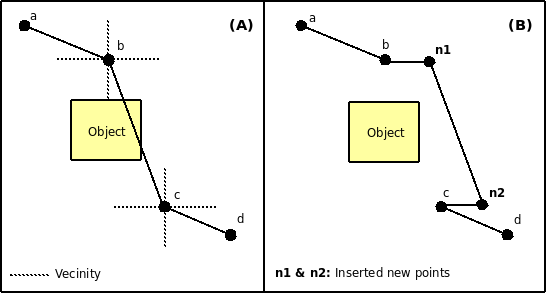
\includegraphics[width=0.5\textwidth]{images/arc}
\caption[The arc operator]{\textbf{The arc operator}. This operator draws an offset value $\Delta$ over a fixed interval called vicinity.
Then, one of the two axes is selected to perform the arc and two new consecutive points are added to the path.
$n_1$ is placed at a $\pm \Delta$ of the point $b$ and $n_2$ at $\pm \Delta$ of point $c$, both of them over the same selected axis.
The axis, sign and value of $\Delta$ are chosen randomly from an uniform distribution.}
\label{fig:arc}
\end{center}
\end{figure}

\begin{figure}[ht]
\begin{center}
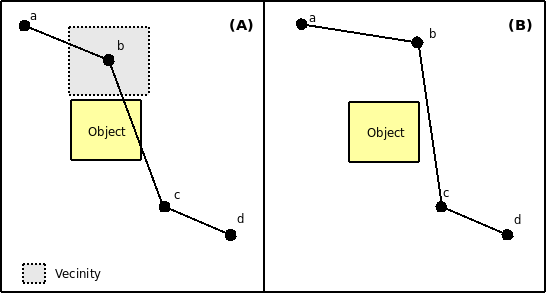
\includegraphics[width=0.5\textwidth]{images/mut}
\caption[The mutation operator]{\textbf{The mutation operator}. This operator draws two offset values $\Delta_x$ and $\Delta_y$ over a vicinity
region. Then the same point $b$ is moved in both axes from $b=[b_x,b_y]$ to $b'=[b_x \pm \Delta_x, b_y\pm \Delta_y]$, where the sign and offset values
are chosen randomly from an uniform distribution.}
\label{fig:mut}
\end{center}
\end{figure}

The second stage is the informed local search,
which is a two step function composed by the \emph{arc} and \emph{mutate} operators
(algorithms~\ref{alg:arc} and~\ref{alg:mut}).
The first one tries to build a square arc around an
obstacle, by inserting two new points between two points in the path that form a
segment colliding with an obstacle, as shown in figure~\ref{fig:arc}.
The second step in the function is a mutation
operator that moves a point close to an obstacle to a
random point in the vicinity, as explained graphically in figure~\ref{fig:mut}.
The mutation operator is inspired by the ones used in the Adaptive Evolutionary
Planner/Navigator (EP/N) presented in~\cite{Xiao97}, while the arc operator is
derived from the arc operator in the Evolutionary Algorithm presented in~%
\cite{Alfaro05}.


\begin{algorithm}[ht]
    \caption{$\operatorname{arc}(\text{path}, \text{firstCol})$}
    \label{alg:arc}
    \begin{algorithmic}[1]
        \STATE \(\text{vicinity} \leftarrow \text{some vicinity size}\)
        \STATE \(\text{randDev} \leftarrow \operatorname{random}(-\text{vicinity},\text{vicinity})\)
        \STATE \(\text{point1} \leftarrow \text{path}[\text{firstCol}]\)
        \STATE \(\text{point2} \leftarrow \text{path}[\text{firstCol}+1]\)
        \IF{\(\operatorname{random}() \% 2\)}
            \STATE \(\text{newPoint1} \leftarrow (\text{point1}[X]+\text{randDev},\text{point1}[Y])\)
            \STATE \(\text{newPoint2} \leftarrow (\text{point2}[X]+\text{randDev},\text{point2}[Y])\)
        \ELSE
            \STATE \(\text{newPoint1} \leftarrow (\text{point1}[X],\text{point1}[Y]+\text{randDev})\)
            \STATE \(\text{newPoint2} \leftarrow (\text{point2}[X],\text{point2}[Y]+\text{randDev})\)
        \ENDIF
        \IF{path segments point1-newPoint1-newPoint2-point2 are collision free}
            \STATE Add new points between point1 and point2
        \ELSE
            \STATE Drop new points
        \ENDIF
    \end{algorithmic}
\end{algorithm}

\begin{algorithm}[ht]
    \caption{$\operatorname{mut}(\text{path}, \text{firstCol})$}
    \label{alg:mut}
    \begin{algorithmic}[1]
        \STATE vicinity $\leftarrow$ some vicinity size
        \STATE path[firstCol][X] $+=$ random$(-\text{vicinity}, \text{vicinity})$
        \STATE path[firstCol][Y] $+=$ random$(-\text{vicinity}, \text{vicinity})$
        \IF{path segments before and after path[firstCol] are collision free}
            \STATE Accept new point
        \ELSE
            \STATE Reject new point
        \ENDIF
    \end{algorithmic}
\end{algorithm}

The third and last stage is the greedy optimization heuristic,
which can be seen as a post-processing for path shortening, that
eliminates intermediate nodes if doing so does not create collisions,
as is described in the algorithm~\ref{alg:postProcess}.

\begin{algorithm}[ht]
    \caption{postProcess$(path)$}
    \label{alg:postProcess}
    \begin{algorithmic}[1]
        \STATE \(i \leftarrow 0\)
        \WHILE{\(i < \operatorname{path.size}() - 2\)}
            \IF{segment \(\operatorname{path}[i]
                \text{\ to\ } \operatorname{path}[i + 2]
                \text{\ is collision free}\)}
                \STATE Delete path[i+1]
            \ELSE
                \STATE \(i \leftarrow i + 1\)
            \ENDIF
        \ENDWHILE
    \end{algorithmic}
\end{algorithm}

